\documentclass{beamer}
\usepackage[french]{babel}
\usepackage[utf8]{inputenc}
\usepackage{amsmath}
\title{Projet de physique Numérique - Allée de Von Karman}
\subtitle{Simulation python}
\author[Cadiou Corentin \and Petit Antoine] % (optional, for multiple authors)
{Cadiou Corentin \and Petit Antoine}
\date{Janvier 2014}
\subject{Physique numérique}

\AtBeginSubsection[]
{
  \begin{frame}
    \frametitle{Table of Contents}
    \tableofcontents[currentsubsection]
  \end{frame}
}

\renewcommand\O{\mathcal{O}}
\begin{document}
  \frame{\titlepage}

  \section{Mise en place de la simulation}
  \subsection{Point de départ}
  \begin{frame}
    \frametitle{Point de départ}
    Code initial : simulation d'une cellule de Rayleigh-Benard.

    Schéma d'advection :
    \begin{itemize}
      \item advection 1/2 lagrangienne -> diffusion (u,v);
      \item advection 1/2 lagrangienne -> diffusion (T);
    \end{itemize}
  \end{frame}
  \begin{frame}
    \frametitle{Point de départ}
    Premières modifications :
    \begin{itemize}
      \item<1-> suppression de la température;
      \item<2-> modification des conditions aux limites:
        \begin{itemize}
          \item<3-> haut et bas : 
            \[ \left. \frac{\partial u}{\partial y}\right|_{y=0,H} = 
            \left. \frac{\partial v}{\partial y}\right|_{y=0,H} = 0 \] 
          \item<4-> droite :
            \[ \left. \frac{\partial u}{\partial x}\right|_{x=W} = 
            \left. \frac{\partial v}{\partial y}\right|_{y=W} = 0 \]
          \item<5-> gauche :
            \[ \left. \frac{\partial u}{\partial x}\right|_{x=0} = u_0
            \qquad \left. \frac{\partial v}{\partial x}\right|_{x=0} = 0\]
        \end{itemize}
    \end{itemize}
  \end{frame}

  \subsection{Incorporation du problème}
  \begin{frame}
    \frametitle{Obstacle}
    Pour commencer, nous avons imposé un obstacle fixe (noté $\O$) :
    \[ \forall (x,y) \in \O : u(x,y) = v(x,y) = 0 \]
    On visualisait en regardant le champ de vitesse \dots
    \begin{center}
      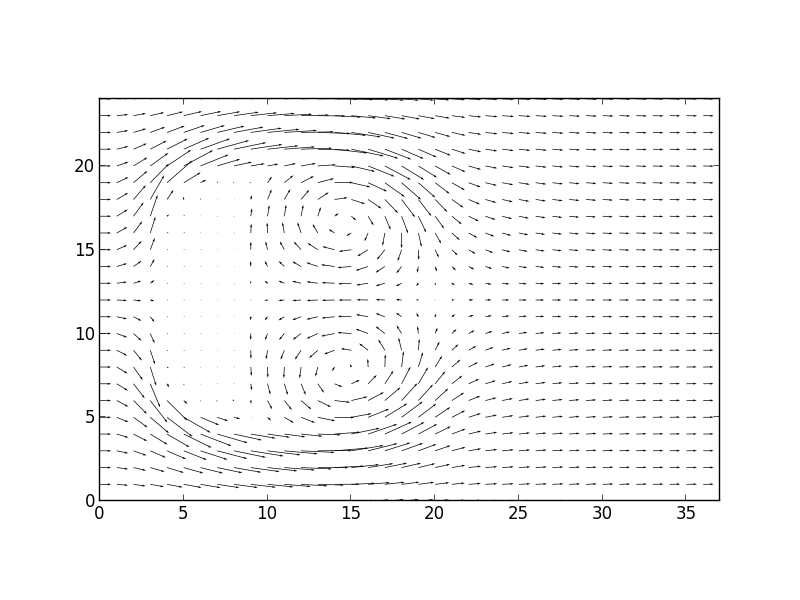
\includegraphics[height=0.6\textheight]{quiver.png}
    \end{center}
  \end{frame}
  \begin{frame}
    \frametitle{Traceurs}
    \dots avant de remplacer cet affichage par la visualisation de
    traceurs, c'est-à-dire un champ supplémentaire noté $T$ advecté et
    passif tel que :
    \begin{align*}
      \forall n\in \mathbb{Z}\quad T(0,n \Delta, t>0) & = 1\\
      \forall (x,y)\quad T(x,y,0) & = 0
    \end{align*}
    \begin{center}
      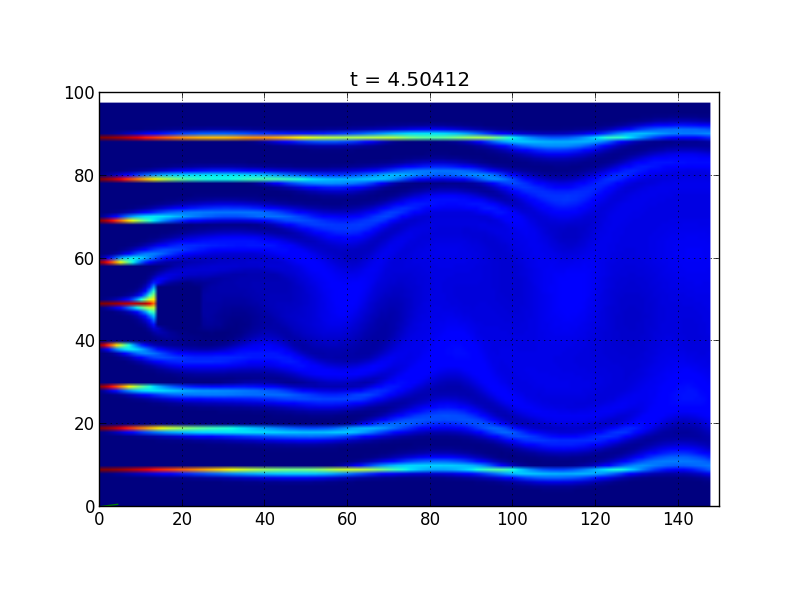
\includegraphics[height=0.6\textheight]{tracer0.png}
    \end{center}
    Ce n'est pas satisfaisant pour observer les tourbillons.
  \end{frame}
  
  \begin{frame}
    \frametitle{Traceurs ``derrière''}
    Idée : l'obstacle impose $\forall (x,y) \in \O: T^n(x,y) = 0$ et on met
    initialement  $\forall (x,y) \not\in \O : T^0 = 1$.
    \begin{center}
%      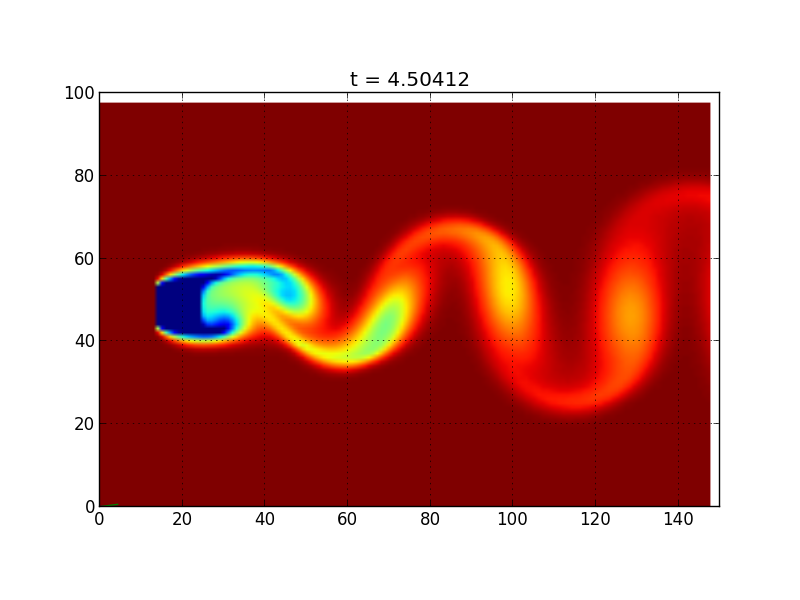
\includegraphics[height=0.6\textheight]{tracer1.png}
    \end{center}
  \end{frame}
  \subsection{BFECC}
  \begin{frame}
    \frametitle{Back and Forth Error Compensation and Correct }
    On effectue les pas suivants pour un champ scalaire $X^n(x,y)$, un
    champ de vitesse $\vec{v}$ et un opérateur d'advection
    $A(\vec{v},X)$ :
    \begin{align}
      X_1 & = A(\vec{v},X^n) \\
      X_2 & = A(-\vec{v},X_1) \\
      X^{n+1} & = A(\vec{v},X - \alpha(X^n - X_2))
    \end{align}
    Dans la littérature, $\alpha = \frac{1}{2}$.
  \end{frame}

  \begin{frame}
    \frametitle{BFECC instable}
    Dans nos conditions (pas de diffusion physique, haut Reynolds)
    : BFECC instable
    \begin{center}
%      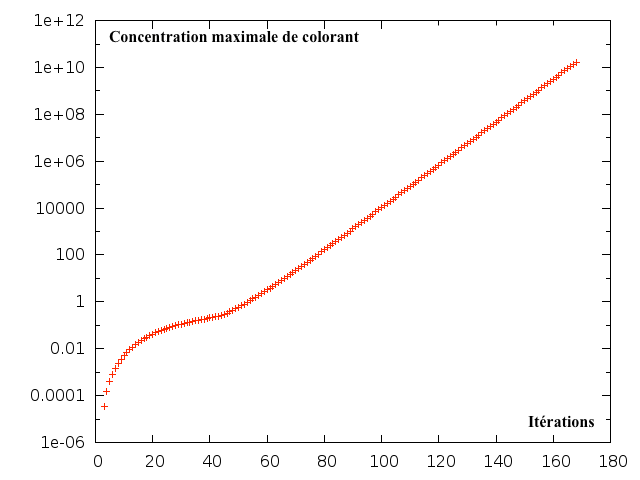
\includegraphics[height=0.8\textheight]{instab_BFECC.png}
    \end{center}
  \end{frame}
  \begin{frame}
    \frametitle{Solution : diminuer $\alpha$}
    Si on diminue $\alpha$, la diffusion numérique augmente :
  \end{frame}
  
  \subsection{L'obstacle qui bouge}
  
\section{Résultats de la simulation}
 
 \subsection{La propulsion}
 		
 	\begin{frame}
 		\frametitle{L'effet de l'amplitude d'oscillation}
 			On fait varier l'amplitude d'oscillation
% 			\centering 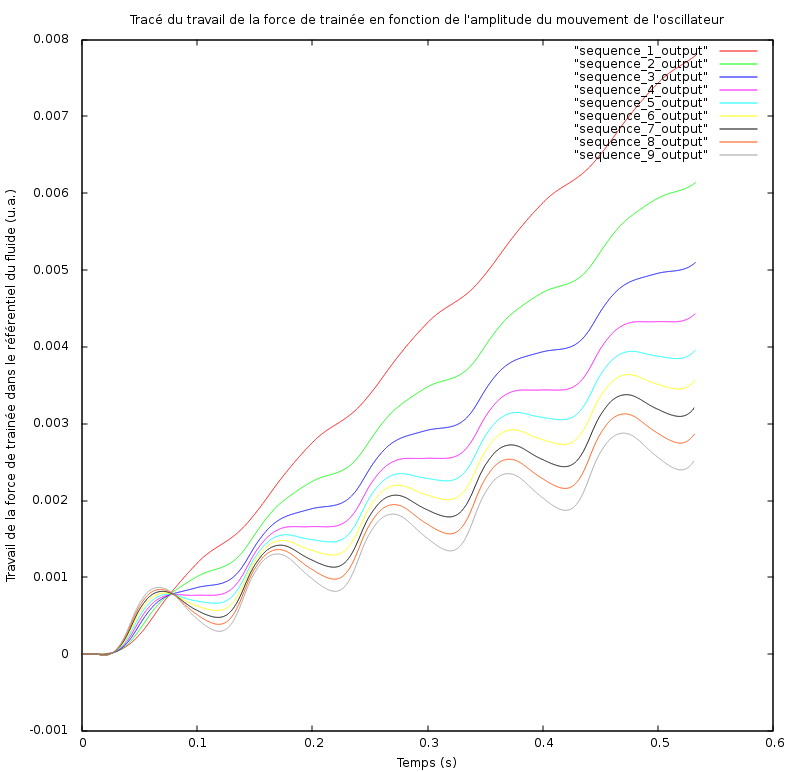
\includegraphics[height= 0.6 \textheight]{9courbes.png}\\
 			Travail de la force de traînée pour une amplitude entre 0,01\degre et 0,09\degre à une fréquence de 10 Hz.
 	\end{frame}
 	
 	\begin{frame}
 		\frametitle{L'effet de l'amplitude d'oscillation}
 		Sur une plus grande plage d'amplitudes, la traînée devient motrice
 %		\centering 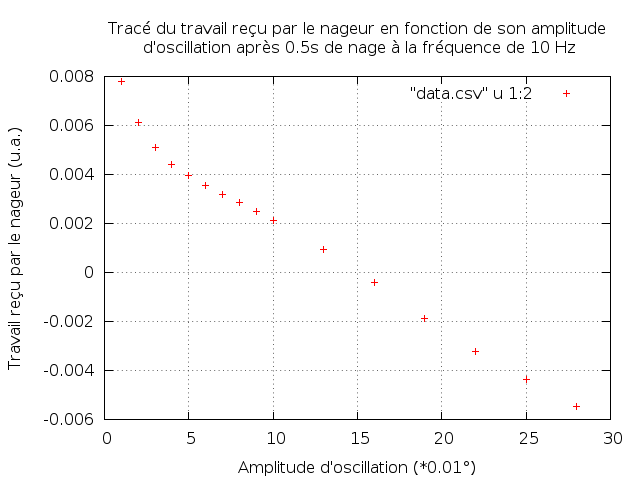
\includegraphics[width= 0.8 \linewidth]{bcp_points.png}\\
 		Travail de la traînée au bout de 2000 itérations
 	\end{frame}
  
  	\begin{frame}
 		\frametitle{Interpolation}
 		On remarque que pour $ \theta_0 < 0,01$, $W_t \propto \theta_0^{-1}$
% 		\centering 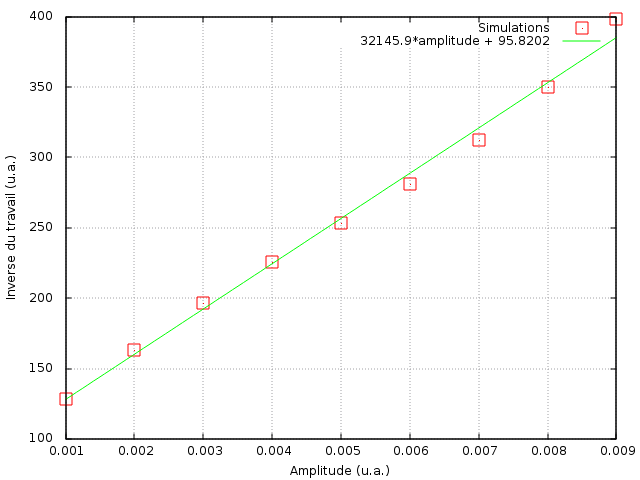
\includegraphics[width= 0.8 \linewidth]{9_courbes_extraites.png}\\
 		Régression linéaire de $W_t^{-1}$ en fonction de $\theta_0$
 	\end{frame}
 	
 	\begin{frame}
 		\frametitle{L'effet de la fréquence d'oscillation}
 			On fait varier la fréquence d'oscillation
 			\centering 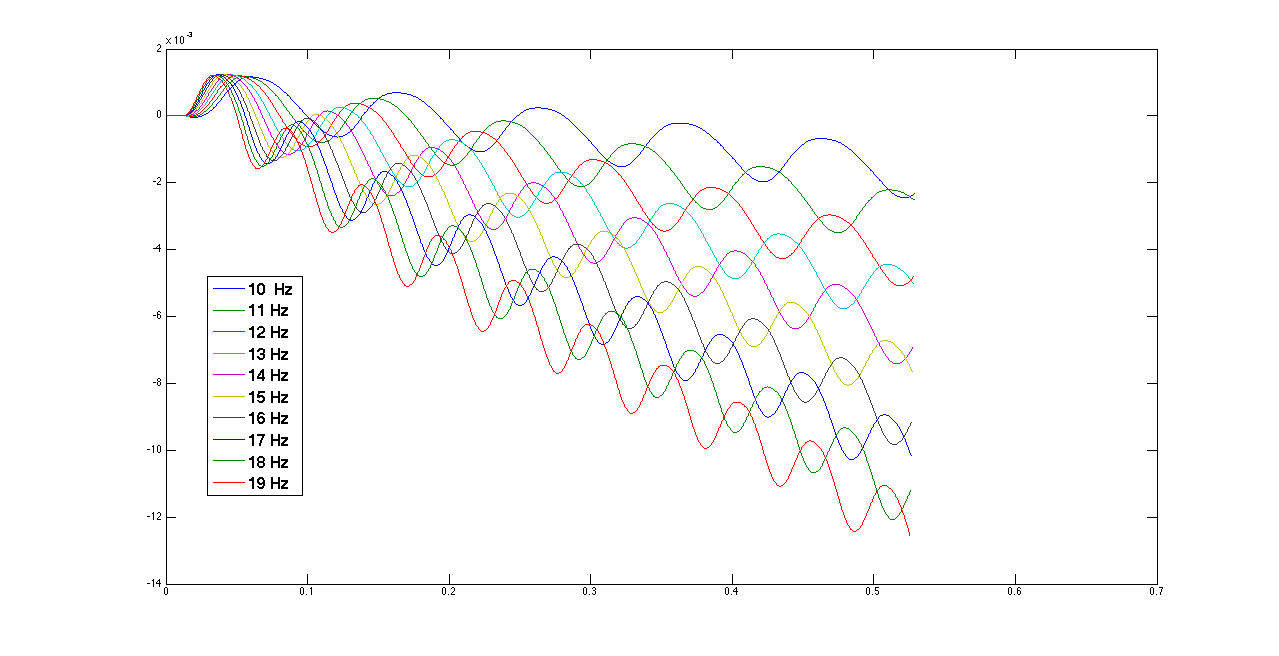
\includegraphics[width= 0.8 \linewidth]{freq0,02.png}\\
 			Travail de la force de traînée pour une fréquence entre 10 Hz et 20 Hz à une amplitude de 0,02\degre.
 	\end{frame}
 	
 	\begin{frame}
 		\frametitle{Interpolation}
 		On interpole la force de traînée moyenne (pentes des droites d'interpolations des droites précédentes)
 		\centering 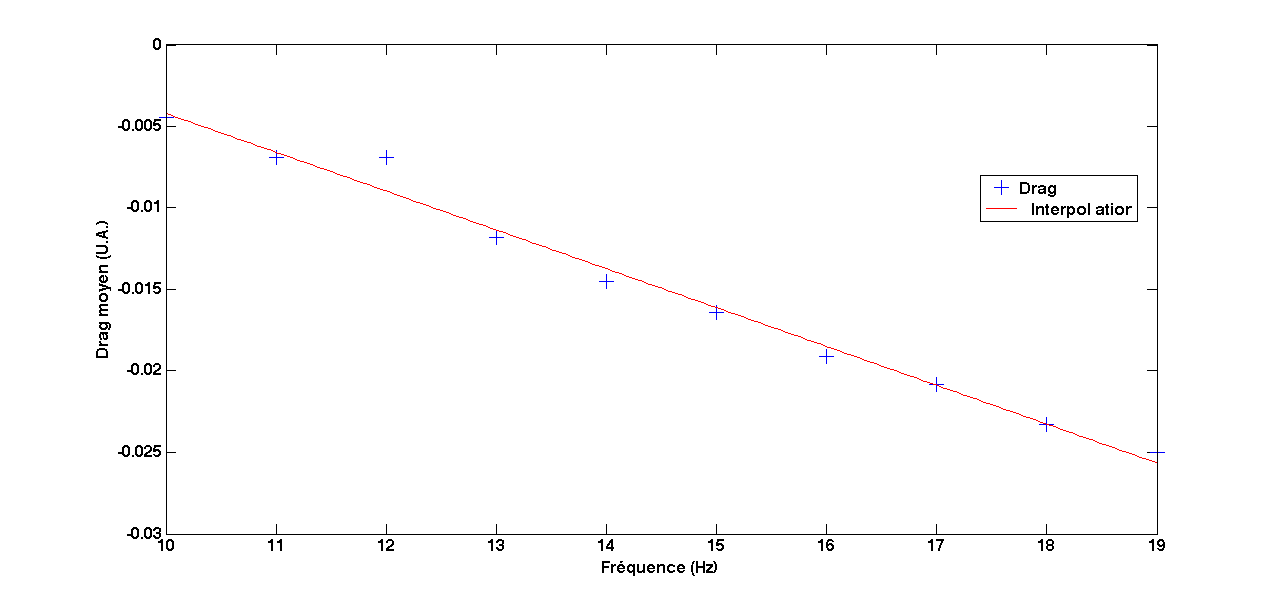
\includegraphics[width= 0.8 \linewidth]{modulationfreq.png} \\
 		La force de traînée est linéaire en fréquence sur la plage étudiée.
 	\end{frame}
\end{document}